\section{Examples} \label{sec:npde.examples}

\subsection{Model evaluation for theophylline PK} \label{sec:exampletheo}

\hskip 18pt The subdirectory {\sf doc} contains a full working example using {\sf npde}. We used the {\sf theopp.tab} dataset provided with {\sf NONMEM} as an example which most users are already familiar with. This dataset is also available under the name {\sf Theoph} in the {\sf dataset} package in {\sf R}, under a slightly different format. This dataset was provided by a study by Dr. Robert Upton of the kinetics of the anti-asthmatic drug theophylline~\cite{NONMEM}.

The subdirectory {\sf doc} contains the following files:
\begin{center}
\begin{tabular} {l l}
\hline
theopp.tab & the observed data \\
simtheopp.tab & the simulated data (with $K$=100)$^1$ \\
fittheop.ctr & the NONMEM control file used for the estimation\\
simultheop.ctr & the NONMEM control file used for the simulations\\
runtheo.res & the result file from the NONMEM estimation \\
theophylline.eps & the graphs \\
theophylline.npde & the file containing the results \\
npde\_userguide.pdf & the present user guide \\
vtrue.dat$^2$ & a file with data simulated under H$_0$ \\
vfalse.dat$^2$ & a file with data simulated assuming a bioavailability divided by 2\\
\hline
\end{tabular}
\end{center}
\noindent$^1$ {\itshape We used K=100 to provide a very quick computation of the $\npde$ and to avoid including a large file in the package, however we recommend using at least K=1000 for the simulations.}

\noindent$^2$ {\itshape These datasets were simulated as examples of external validation datasets in~\cite{CometsCMPB08}}

%\newpage
\subsubsection{Data}

\hskip 18pt Theophylline concentrations were measured in 12 patients over a period of 24~hr after a single oral dose of the drug. Each patient received a different dose. The data file has the following structure:
\begin{center}
\begin{tabular} {l c c c c c}
\hline
Column number & 1 & 2 & 3 & 4 & 5 \\
Column name & ID & Dose & Time & Conc & Wt \\
Item meaning & Patient id & Dose & Time & Concentrations & Weight \\
\hline
\end{tabular}
\end{center}
Doses are given in~mg, times in hours and concentrations are reported in mg.L$^{-1}$.

Figure~\ref{fig:theodata} displays the dataset. The data for the first two patients is given in the appendix (see page~\pageref{sec:appdata}), to show the format of the data file.
\begin{figure}[!h]
\par\kern -0.3cm
\begin{center}
\epsfig{file=/home/eco/work/npde/npde30/latexDoc/figsDev/doc_theodata_gg.eps,width=13cm}
\end{center}
\caption{Theophylline data.}\label{fig:theodata}
\end{figure}

\subsubsection{Model}

\hskip 18pt The data was analysed with a one-compartment model with first-order absorption and elimination, parameterised in absorption rate constant k$_a$ (units hr$^{-1}$) volume of distribution V (units L) and elimination rate constant k (units hr$^{-1}$). Concentrations at time 0 were removed from the dataset. The model did not include covariates. Interindividual variability was modelled using an exponential model for the three pharmacokinetic parameters. A covariance between the parameters k and V was assumed, yielding the following variance-covariance matrix:
\begin{equation}
\Omega=\left(
\begin{array}{ccc}
\omega_{k_a}^2 & 0 & 0\\
0 & \omega_{V}^2 & omega_{k,V}={\rm cov}(\eta_{k},\eta_{V}) \\
0 & {\rm cov}(\eta_{k},\eta_{V}) & \omega_{k}^2\\
\end{array}
\right)
\end{equation}
The residual error model was a combined additive and proportional
error model as in equation~\ref{eq:errormod}.

\bigskip These data were analysed with the software {\sf NONMEM} version 5.1. The ADVAN2 routine was used. The estimation method was the {\sf FOCE} algorithm with the {\sf INTERACTION} option. The control file is given in the Appendix (see page~\pageref{sec:appanalctr}) and the relevant results in the ouput file {\sf runtheo.res} are shown on page~\pageref{sec:appresnonmem}.

The following parameter estimates were obtained:
\begin{center}
\begin{tabular} {l c | l c}
\hline 
\multicolumn{2}{c}{Population mean} & \multicolumn{2}{c}{Interindividual
variability (CV\%)} \\
\hline 
k$_a$ (hr$^{-1}$) & 1.51 & $\omega_{k_a}$ (-) & 0.67 \\
V (L) & 0.46 & $\omega_{V}$ (-) & 0.12 \\
k (L.hr$^{-1}$) & 0.087 & $\omega_{k}$ (-) & 0.13 \\
$\sigma_{\rm inter}$ (mg.L$^{-1}$) & 0.088 & cor$(\eta_{k},\eta_{V})$ (-) & 0.99 \\
$\sigma_{\rm slope}$ (-) & 0.26 & &\\
\hline
\end{tabular}
\end{center}

\subsubsection{Simulations}

\hskip 18pt The simulations were also performed using {\sf NONMEM} version 5.1. The control file used for the simulations is given in the Appendix (see page~\pageref{sec:appsimulctr}). The beginning is identical to the control file used for the analysis (page~\pageref{sec:appresnonmem}); the initial values in the {\sf \$THETA}, {\sf \$OMEGA}, {\sf \$SIGMA} blocks have been changed to the values estimated with the model, the {\sf \$ERROR} block includes a line to output the simulated data, and the {\sf \$TABLE} block has been changed to output the simulated data in a file.

The number of simulations can be changed with the {\sf SUBPROBLEMS} options in the {\sf \$SIMULATION} block. Here, we use 100 simulations to compute the $\npde$ quickly as an illustration, but larger numbers are more appropriate (we recommend at least 1000 simulations). Simulations were saved in the file {\sf simtheopp.tab}.

\subsubsection{Computing $\npde$} \label{sec:expde}

\hskip 18pt The interactive version of the program was run below. In a first step, the user was prompted to enter all details necessary for the computations (text \textcolor{mycol}{\bf in purple} show values entered by the user while text in black is printed by the program):

\bigskip
{\sf
\noindent myres<-npde() \\
Name of the file containing the observed data: \textcolor{mycol}{\bf theopp.tab}\\
Automatic recognition of columns in the dataset (y/Y) [default=yes] ? \textcolor{mycol}{\bf n}\\
I'm assuming file theopp.tab has the following structure:\\
$\phantom{me}$\hskip 0.5cm        ID X Y ...\\
and does not contain a column signaling missing data.\\
To keep, press ENTER, to change, type any letter: \textcolor{mycol}{\bf n}\\
$\phantom{me}$\hskip 0.5cm Column with ID information ? \textcolor{mycol}{\bf 1}\\
$\phantom{me}$\hskip 0.5cm Column with X (eg time) information ? \textcolor{mycol}{\bf 3}\\
$\phantom{me}$\hskip 0.5cm Column with Y (eg DV) information ? \textcolor{mycol}{\bf 4}\\
$\phantom{me}$\hskip 0.5cm Column signaling missing data (eg MDV, press ENTER if none) ? \\
$\phantom{me}$\hskip 0.5cm Column signaling censoring (eg CENS, press ENTER if none) ? \\
$\phantom{me}$\hskip 0.5cm Column with individual predictions (eg ipred, press ENTER if none) ?  \\
$\phantom{me}$\hskip 0.5cm Columns with covariates (eg WT; enter one at a time, press ENTER if none or when finished) ?  \\
Name of the file containing the simulated data: \textcolor{mycol}{\bf 
simtheopp.tab}\\
Do you want results and graphs to be saved to files (y/Y) [default=yes] ? \textcolor{mycol}{\bf y}\\
Different formats of graphs are possible:\\
$\phantom{me}$\hskip 0.5cm         1. Postscript (extension eps)\\
$\phantom{me}$\hskip 0.5cm         2. JPEG (extension jpeg)\\
$\phantom{me}$\hskip 0.5cm         3. PNG (extension png)\\
$\phantom{me}$\hskip 0.5cm         4. Acrobat PDF (extension pdf)\\
Which format would you like for the graph (1-4) ? \textcolor{mycol}{\bf 1}\\
Name of the file (extension will be added, default=output): 
\textcolor{mycol}{\bf theophylline}\\
Do you want to compute npde (y/Y) [default=yes] ? \textcolor{mycol}{\bf y}\\
Do you want to compute pd (y/Y) [default=yes] ? \textcolor{mycol}{\bf y}\\
Different decorrelation methods are available:\\
$\phantom{me}$\hskip 0.5cm         1. Cholesky decomposition (default)\\
$\phantom{me}$\hskip 0.5cm         2. Inverse using diagonalisation (as in Monolix and Nonmem)\\
$\phantom{me}$\hskip 0.5cm         3. Cholesky followed by polar decomposition\\
Which method should be used for the decorrelation (1-3) ? \textcolor{mycol}{\bf 1}\\
Method used to handle censored observations:\\
$\phantom{me}$\hskip 0.5cm         1. omit: pd will be set to NaN for missing data\\
$\phantom{me}$\hskip 0.5cm         2. cdf: pd will be imputed using a random sample from U(0,p\_LOQ) where p\_LOQ is the probability, according to the model, that a given observation is less than LOQ (default)\\
$\phantom{me}$\hskip 0.5cm         3. loq: an observation below the LOQ will be imputed to the LOQ\\
$\phantom{me}$\hskip 0.5cm         4. ypred: an observation below the LOQ will be imputed to the population model prediction\\
$\phantom{me}$\hskip 0.5cm         5. ipred: an observation below the LOQ will be imputed to the individual model prediction\\
Which method should be used (1-5) ? \textcolor{mycol}{\bf 2}\\
Do you want a message printed as the computation of npde begins in a new
subject (y/Y) [default=no] ? \textcolor{mycol}{\bf y}\\
Do you want the function to return an object (y/Y) [default=yes] ? \textcolor{mycol}{\bf y}\\
}

In the second step, the program computed the normalised prediction distribution errors, plotted the corresponding graphs and performed the statistical tests for $\npde$, then computed the prediction discrepancies (for which no tests are reported). A warning is issued here because the number of simulations is considered too small. 

Here we see that the test of the mean (\texttt{t-test}) and variance (\texttt{Fisher variance test}) don't shown any significant departure from the theoretical values of 0 and 1 respectively, on the other hand, the normality test (\texttt{SW test of normality}) indicates a departure from the normal distribution, so that the global test (\texttt{Global adjusted p-value}), consisting of a Bonferroni-corrected combination of the three test, also shows a significant departure from the theoretical distribution. However, the results of the tests don't necessarily reflect model adequacy in this case, because of the small number of simulations used.
%\newpage
{\small
\begin{verbatim}
Automatic detection of variables is ON. The program will attempt to detect
both mandatory variables (ID, X, Y) and optional variables (IPRED, MDV, CENS) 
when they are not specifically given or when the user-specified names are not 
found in the dataset, by looking in the names of the columns (to override this 
behaviour, please use argument detect=FALSE in the call to npdeData().
Reading data from file ../data/theopp.tab 
These are the first lines of the dataset as read into R. Please check the format 
of the data is appropriate, if not, modify the na and/or sep items and retry:
  ID Dose Time  Conc   Wt
1  1 4.02 0.00    NA 79.6
2  1   NA 0.25  2.84   NA
3  1   NA 0.57  6.57   NA
4  1   NA 1.12 10.50   NA
5  1   NA 2.02  9.66   NA
6  1   NA 3.82  8.58   NA

The following NpdeData object was successfully created:
Object of class NpdeData
    longitudinal data
Dataset ../data/theopp.tab 
    Structured data: Conc ~ Time | ID 
    predictor: Time (hr) 
NpdeDataReading data from file ../data/simtheopp.tab 
These are the first lines of the dataset as read into R. Please check the format 
of the data is appropriate, if not, modify the na and/or sep items and retry:
  ID xsim      ysim
1  1 0.00 -0.090212
2  1 0.25  2.289200
3  1 0.57  4.227900
4  1 1.12  5.497900
5  1 2.02  7.917300
6  1 3.82  5.394300
There are rows with MDV=1 in the original dataset, the corresponding rows 
will be removed from the simulated dataset.

Warning: the number of simulations is 100 which may be too small.
We advise performing at least 1000 simulations to compute npde.
Computing the npde for subject  1 
Computing the npde for subject  2 
Computing the npde for subject  3 
Computing the npde for subject  4 
Computing the npde for subject  5 
Computing the npde for subject  6 
Computing the npde for subject  7 
Computing the npde for subject  8 
Computing the npde for subject  9 
Computing the npde for subject  10 
Computing the npde for subject  11 
Computing the npde for subject  12 

---------------------------------------------
Distribution of npde :
      nb of obs: 120 
           mean= 0.0668   (SE= 0.095 )
       variance= 1.074   (SE= 0.14 )
       skewness= 0.511 
       kurtosis= 0.2912 
---------------------------------------------

Statistical tests (adjusted p-values):
  t-test                : 1
  Fisher variance test  : 1
  SW test of normality  : 0.00819 **
  Global test           : 0.00819 **
---
Signif. codes: '***' 0.001 '**' 0.01 '*' 0.05 '.' 0.1 
---------------------------------------------
\end{verbatim}
}

\paragraph{Note:} the p-values are now all presented after adjustement with a Bonferroni correction. In the previous versions of {\sf npde} only the global test was adjusted, while the other p-values were presented as raw values. We have now changed this for consistency.

%\begin{verbatim}
% Previously... why changed ??? (including mean & moments => check computation)
% Saving graphs in file keepnpde/inst/doc/theophylline.eps 
% ---------------------------------------------
% Distribution of npde:
%            mean= 0.05641   (SE= 0.092 )
%        variance= 1.024   (SE= 0.13 )
%        skewness= 0.4065 
%        kurtosis= 0.0888 
% ---------------------------------------------
% 
% Statistical tests
%   Wilcoxon signed rank test  : 0.883
%   Fisher variance test       : 0.823
%   SW test of normality       : 0.00509 **
% Global adjusted p-value      : 0.0153 *
% ---
% Signif. codes: '***' 0.001 '**' 0.01 '*' 0.05 '.' 0.1 
% ---------------------------------------------
% Computing pd
% Saving results in file keepnpde/inst/doc/theophylline.npde 
%\end{verbatim}


\bigskip
Alternatively, the first step can be run non-interactively, with the following command:
\begin{verbatim}
myres<-autonpde("theopp.tab","simtheopp.tab",1,3,4,namsav="theophylline",
verbose=TRUE)
\end{verbatim}

%The results of the statistical tests show that the normality assumption for the normalised prediction distribution errors is rejected according to the Shapiro-Wilks test for normality, as can be seen in the plots in the next section (figure~\ref{fig:respde}). The adjusted p-value for the 3 tests taken simultaneously using a Bonferroni correction therefore rejects the assumption that the model describes the data adequately. 

%\newpage
\subsubsection{Graphs}

\hskip 18pt The graphs in figure~\ref{fig:respde} are plotted in a window, and saved to a file (unless {\sf boolsave=F}).
\begin{figure}[!h]
\par\kern -0.3cm
\begin{center}
\epsfig{file=/home/eco/work/npde/npde30/latexDoc/figsDev/doc_theodefault_gg.eps,width=14cm}
\end{center}
\caption{Graphs plotted by the {\sf npde()} or {\sf autonpde()}
functions.}\label{fig:respde}
\end{figure}
The quantile-quantile plot and the histogram show a group of values corresponding to $\npde=2.33$, corresponding to predicted distribution errors set at 0.99, and the prediction bands shows the corresponding departure graphically on the two upper graphs. This indicates observations larger than all the 100 corresponding simulated values. This often happens when $K$ is small as is the case in this example (K=100), and can explain the departure from normality seen in the tests. However, even increasing the number of simulations to 1000 or 2000 does not in this example yield a non-significant test, meaning the model does not describe the data adequately (results not shown).

In the scatterplots (lower two graphs), the pink area is the prediction interval for the median, while the blue areas shows the prediction areas for the boundaries of the 95\% prediction intervals. The prediction bands are very large because of the small number of simulations so that model misspecification is not so obvious. By default, the binning on the X-axis uses bins of equal size (number of observations), and the mean of the X values in the bin is used to plot the bin, which explains why the bins do not extend to the largest X-value especially in the lower right plot, but this default behaviour can be tuned in the options.

Figure~\ref{fig:theovpc} shows the VPC, where the prediction bands are again very large because of the low number of simulations.
\begin{figure}[!h]
\par\kern -0.3cm
\begin{center}
\epsfig{file=/home/eco/work/npde/npde30/latexDoc/figsDev/doc_theovpc_gg.eps,width=13cm}
\end{center}
\caption{VPC of the theophylline data, with 100 simulated datasets.}\label{fig:theovpc}
\end{figure}

\newpage
\subsubsection{Tests}

\hskip 18pt A method {\sf gof.test()} is available for objects of class \texttt{NpdeObject}. When applied to the object resulting from a call to {\sf npde()} or {\sf autonpde()}, it will produce the same results as previously:
\begin{verbatim}
---------------------------------------------
Distribution of npde :
      nb of obs: 120 
           mean= 0.0668   (SE= 0.095 )
       variance= 1.074   (SE= 0.14 )
       skewness= 0.511 
       kurtosis= 0.2912 
---------------------------------------------

Statistical tests (adjusted p-values):
  t-test                : 1
  Fisher variance test  : 1
  SW test of normality  : 0.00819 **
  Global test           : 0.00819 **
---
Signif. codes: '***' 0.001 '**' 0.01 '*' 0.05 '.' 0.1 
---------------------------------------------
\end{verbatim}
Here, the four p-values are redirected to the R object {\sf y}. With the option {\sf which="pd"} (resp. 'pd'), the user can select tests for the $\pd$ (resp. $\npd$) instead of the $\npde$, but the tests will only be strictly valid when there is only one observation per subject, otherwise the test incurrs a significant increase in type I error~\cite{MentrePDE, Brendel06}.

A {\sf gof.test()} method has also been defined for numeric vectors, in which case it will compute the first moments and perform the four tests. The statistical diagnostics can therefore be regenerated easily without running the computation all over again, provided the results have been saved. In the example above, the $\npde$ were saved to a file named {\sf theophylline.npde}. The following code reads the results from this file and computes the same tests as above:
\begin{verbatim}
dat<-read.table("theophylline.npde",header=T)
y<-gof.test(dat$npde) 
\end{verbatim}

% Ici parler de la correction de Bonferroni versus la correction de Simes?
% ou bien préparer une fonction pour calculer la p-value avec une correction de
% Simes?

\clearpage

\subsection{Model evaluation for viral loads in HIV (with BQL data)} \label{sec:PDexample}

\hskip 18pt In this example, we use simulated datasets based on a real study of viral load in HIV patients. The real data and model were obtained in a phase II clinical trial supported by the French Agency for AIDS Research, the COPHAR 3 - ANRS 134 trial~\cite{GoujardISA2010}. The simulated datasets available in the library were generated in a simulation study designed to evaluate the new method proposed to handle BQL data~\cite{Nguyen2012}. Data was simulated using a simple bi-exponential HIV dynamic model describing the two-phase decline of viral load during anti-retroviral treatment; the dataset was then censored at different LOQ levels (LOQ=20 or 50~copies/mL) to generate two datasets containing two different proportions of BQL data.

The {\sf data} subdirectory contains the following files:
\begin{center}
\begin{tabular} {l l}
\hline
virload.tab & simulated validation dataset without BQL observations \\
virload20.tab & simulated validation dataset with LOQ=20 copies/mL \\
virload50.tab & simulated validation dataset with LOQ=50 copies/mL\\
simvirload.tab & simulated Monte Carlo samples (with $K$=1000) \\
\hline
\end{tabular}
\end{center}
The actual proportion of BQL data in the real dataset was 48\%, while the proportion of BQL data in the censored datasets is respectively 26 and 44\% for virload20.tab and virload50.tab.

%\newpage
\subsubsection{Data}

\hskip 18pt Each dataset contains 50 patients sampled 6 times over a treatment period of 24 weeks (day 0, 28, 56, 84, 112, 168). Individual model predictions were obtained from a fit of the model described in the next section to showcase the different censoring methods. The data file has the following structure:
\begin{center}
\begin{tabular} {l c c c c c}
\hline
Column number & 1 & 2 & 3 & 4 & 5\\
Column name & ID & Time & Log\_VL & cens & ipred \\
Item meaning & ID & Time & log$_{10}$(viral load) & Censored or not & individual predictions \\
\hline
\end{tabular}
\end{center}
Time is in days and viral loads are reported in log$_{10}$ of the values measured in copies/mL.

\subsubsection{Model and parameters for simulation}

\hskip 18pt The model used in this example is a bi-exponential model which was proposed by Ding and colleagues~\cite{Ding1999}, where the model $f$ used to describe the evolution of log$_{10}$(viral load) is given by:
\begin{equation}
f(t_{ij},\theta_{i})=\log_{10}(P_{1i}\mbox{e}^{-\lambda_{1i}t_{ij}}+P_{2i}\mbox{e}^{-\lambda_{2i}t_{ij}})
\end{equation}
This model contains four individual parameters $\theta_{i}$: $P_{1i}$, $P_{2i}$ are the baseline values of viral load and the $\lambda_{1i}$, $\lambda_{2i}$ represent the biphasic viral decline rates. These parameters are positive and assumed to follow a log-normal distribution with fixed effects $\mu=(P_{1},P_{2},\lambda_{1},\lambda_{2})$. A correlation between the random effects of $P_{1},$ $P_{2}$ and a constant error model were found on real data. The values used for simulation are inspired by the parameters obtained when analysing real data collected in the COPHAR 3 - ANRS 134 trials~\cite{GoujardISA2010}, and are given in the following table:

\begin{center}
\begin{tabular} {l c | l c}
\hline 
\multicolumn{2}{c}{Population mean} & \multicolumn{2}{c}{Interindividual variability (CV\%)} \\
\hline 
P$_1$ (copies/mL) & 25000 & $\omega_{P_1}$ (-) & 2.1 \\
P$_2$ (copies/mL) & 250 & $\omega_{P_1}$ (-) & 1.4 \\
$\lambda_1$ (day$^{-1}$) & 0.2 & $\omega_{\lambda_1}$ (-) & 0.3 \\
$\lambda_2$ (day$^{-1}$) & 0.02 & $\omega_{\lambda_2}$ (-) & 0.3 \\
$\sigma $ (log$_{10}$(copies/mL)) & 0.14 & cor$(\eta_{P_1},\eta_{P_2})$ (-) & 0.8 \\
\hline
\end{tabular}
\end{center}

\subsubsection{Computing npde in the presence of BQL data}

\hskip 18pt The following code was used to compute the npde for the 3 datasets. For the two censored datasets, censored data were either omitted (option \texttt{cens.method="omit"}) or imputed as described in Methods (default, option \texttt{cens.method="cdf"}).

\begin{verbatim}
data(virload)
data(simvirload)
xviroad<-autonpde(namobs=virload,namsim=simvirload,boolsave=FALSE, 
units=list(x="days",y="copies/mL"))

data(virload20)
x20<-autonpde(namobs=virload20,namsim=simvirload,boolsave=FALSE, 
units=list(x="days",y="copies/mL"))
x20.omit<-autonpde(namobs=virload20,namsim=simvirload,boolsave=FALSE, 
units=list(x="days",y="copies/mL"),cens.method="omit")

data(virload50)
x50<-autonpde(namobs=virload50,namsim=simvirload,boolsave=FALSE, 
units=list(x="days",y="copies/mL"))
x50.omit<-autonpde(namobs=virload50,namsim=simvirload,boolsave=FALSE, 
units=list(x="days",y="copies/mL"),cens.method="omit")
\end{verbatim}

A simulation study was performed in~\cite{Nguyen2012} to assess the performance of the method implemented in the new version of \texttt{npde}. The simulation study showed increased power to detect model misspecification, compared to simply omitting BQL data from the dataset. As expected, we observe a decrease in power when the proportion of BQL increases, since the imputation is based on the model.

\subsubsection{Graphs}

\hskip 18pt The plot function produces by default the 4 graphs shown in figure~\ref{fig:respde}. A number of graphs have been defined, which can be individually accessed through the \texttt{plot.type} option.

\paragraph{Data:} Figure~\ref{fig:x50.data} shows a plot of the data for the dataset with the highest level of censoring (LOQ=50~cp/mL), obtained by selecting the 'data' \texttt{plot.type}. By default, the imputed data will be plotted as red stars, completing the observed dataset (top left plot). Options are available to remove the BQL data from the plot (option \texttt{plot.loq=FALSE}, top right) or to plot them at the censoring value (option \texttt{impute.loq=FALSE}, bottom left). 

\begin{figure}[!h]
\par\kern -0.3cm
\begin{center}
\epsfig{file=/home/eco/work/npde/npde30/latexDoc/figsDev/doc_data50_gg.eps,width=14cm}
\end{center}
\caption{Figure showing the data, with different options. The default is shown top left, and plots the BQL data using the imputed values. Other options are to remove the BQL data from the plot (top right) or to plot them at the value used for censoring (bottom left). A dotted line shows the LOQ.}\label{fig:x50.data}
\end{figure}

The following code was used to produce this figure. Each plot is stored in an object, and the {\sf grid.arrange()} function from the {\sf grid} package is used to produce a user-defined layout (here, 2 by 2):
\begin{verbatim}
x1<-plot(x50, plot.type="data", xlab="Time (hr)", ylab="log(Viral load) (cp/mL)", line.loq=TRUE, ylim=c(0,6.5), main="LOQ imupted using cdf")
x2<-plot(x50, plot.type="data", xlab="Time (hr)", ylab="log(Viral load) (cp/mL)", plot.loq=FALSE, line.loq=TRUE, ylim=c(0,6.5), main="LOQ removed from plot")
x3<-plot(x50, plot.type="data", xlab="Time (hr)", ylab="log(Viral load) (cp/mL)", impute.loq=FALSE, line.loq=TRUE, ylim=c(0,6.5), main="LOQ as in dataset before imputation")
x4<-plot(x50.ipred, plot.type="data", xlab="Time (hr)", ylab="log(Viral load) (cp/mL)", line.loq=TRUE, ylim=c(0,6.5), main="LOQ imputed to individual prediction")

grid.arrange(grobs=list(x1,x2,x3,x4), nrow=2, ncol=2)
\end{verbatim} 

\paragraph{Comparing the censoring methods:} in this section, we compare the different censoring methods for the dataset with a high censoring value (virload50). By default, the imputation method described in section~\ref{sec:npde} is used, yielding the plots in figure~\ref{fig:x50.cdf}. With the {\sf omit} censoring method, censored values are omitted from the graph altogether (figure~\ref{fig:x50.omit}). With the {\sf ipred} or {\sf ppred} censoring methods, censored values are replaced by population or individual predictions (figure~\ref{fig:x50.ipred} and~\ref{fig:x50.ppred}).

\begin{figure}[!h]
\par\kern -0.3cm
\begin{center}
\epsfig{file=/home/eco/work/npde/npde30/latexDoc/figsDev/x50_cdf_gg.eps,width=14cm}
\end{center}
\par\kern -0.3cm
\caption{Default graphs for the virload50 dataset, default censoring method ({\sf "cdf"}).}\label{fig:x50.cdf}
\end{figure}

\begin{figure}[!h]
\par\kern -0.5cm
\begin{center}
\epsfig{file=/home/eco/work/npde/npde30/latexDoc/figsDev/x50_omit_gg.eps,width=14cm}
\end{center}
\par\kern -0.5cm
\caption{Default graphs for the virload50 dataset, censoring method {\sf "omit"}.}\label{fig:x50.omit}
\end{figure}

\begin{figure}[!h]
\par\kern -0.5cm
\begin{center}
\epsfig{file=/home/eco/work/npde/npde30/latexDoc/figsDev/x50_ipred_gg.eps,width=14cm}
\end{center}
\par\kern -0.5cm
\caption{Default graphs for the virload50 dataset, censoring method {\sf "ipred"}.}\label{fig:x50.ipred}
\end{figure}

\clearpage
\begin{figure}[!h]
\par\kern -0.5cm
\begin{center}
\epsfig{file=/home/eco/work/npde/npde30/latexDoc/figsDev/x50_ppred_gg.eps, width=14cm}
\end{center}
\par\kern -0.5cm
\caption{Default graphs for the virload50 dataset, censoring method {\sf "ppred"}.}\label{fig:x50.ppred}
\end{figure}

%\clearpage
\paragraph{VPC:} The Visual Predictive Check (VPC) for the data without and with imputation is shown in figure~\ref{fig:x50.vpc}.

\begin{figure}[!h]
\par\kern -0.2cm
\begin{center}
\epsfig{file=/home/eco/work/npde/npde30/latexDoc/figsDev/userwaffle_vpc.eps,width=14cm}
\end{center}
\caption{VPC obtained by removing BQL values (left) and by imputing them (right), for the dataset where LOQ=50 cp/mL. A dotted line shows the LOQ.}\label{fig:x50.vpc}
\end{figure}
\clearpage

Figure~\ref{fig:x50.ploq} shows the probability of being LOQ according to the model, with the corresponding prediction interval.
\begin{figure}[!h]
\par\kern -0.3cm
\begin{center}
\epsfig{file=/home/eco/work/npde/npde30/latexDoc/figsDev/virload_ploq_gg.eps, width=10cm}
\end{center}
\caption{Probability of being LOQ according to the model.}\label{fig:x50.ploq}
\end{figure}

These two figures can be obtained by the following code:
\begin{verbatim}
vpc.omit<-plot(x50.omit,plot.type="vpc")
vpc.cdf<-plot(x50,plot.type="vpc")
grid.arrange(grobs=list(vpc.omit, vpc.cdf), nrow=1, ncol=2)

plot(x50,plot.type="loq")
\end{verbatim} 

\clearpage
\paragraph{Scatterplots:} Scatterplots of npde or pd versus time or predictions are available. An example is given in figure~\ref{fig:x50.xscatter} for npde versus time, with or without imputation. Here imputing the censored values works very well, as can be expected given that the true model was used to simulate the data.

\begin{figure}[!h]
\par\kern -0.2cm
\begin{center}
\epsfig{file=/home/eco/work/npde/npde30/latexDoc/figsDev/userwaffle_xscatter.eps,width=14cm}
\end{center}
\par\kern -7cm
\caption{Scatterplots obtained by removing BQL values (left) and by imputing them (right), for the dataset where LOQ=50 cp/mL. A dotted line shows the LOQ.}\label{fig:x50.xscatter}
\end{figure}

This figure can be obtained by the following code:
\begin{verbatim}
xscatter.omit<-plot(x50.omit,plot.type="x.scatter")
xscatter.cdf<-plot(x50,plot.type="x.scatter")
grid.arrange(grobs=list(xscatter.omit, xscatter.cdf), nrow=1, ncol=2)
\end{verbatim} 

\clearpage
\subsection{Model evaluation for warfarin PK} \label{sec:warfarin}

\subsubsection{Data}

\hskip 18pt The warfarin dataset~\cite{OReilly68} was collected in a study on warfarin. The dataset contains 32 series of pharmacokinetic measurements after a single dose of 1.5~mg/kg in 30 healthy subjects (two were sampled twice but the occasions are treated as separate subjects in the analyses made using this data). 
The {\sf warfarin} data frame has 251 rows and 8 columns of data containing data on the pharmacokinetics of warfarin, an anticoagulant drug used in the prevention of thrombosis and thromboembolism. It represents the PK part of a larger dataset including both warfarin concentrations and prothrombin complex activity (PCA), which measures the decreased coagulation  activity resulting from the inhibition of vitamin K recycling, the mechanism of  action of warfarin. The subjects in the study were sampled at different times over a period of up to 120 hours.

The data is distributed with the {\sf Monolix} software as a demo for PK/PD modelling. We slightly reformated it for R, removing the line at time=0 and filling the {\sf amt} column with the dose for each subject. The data is shown in figure~\ref{fig:warfarin.data}.

\begin{figure}[!h]
\par\kern -0.2cm
\begin{center}
\epsfig{file=/home/eco/work/npde/npde30/latexDoc/figsDev/doc_warfarin_data.eps,width=12cm}
\end{center}
\caption{Warfarin data}\label{fig:warfarin.data}
\end{figure}


We used the base model reported in the case-study from the {\sf Monolix} documentation, and built a covariate model using a stepwise strategy for the purpose of showcasing covariate graphs in the {\sf npde} library.  The PK model was a two-compartment model, with first-order absorption and a time-delay. Interindividual variability was modelled as log-normal distributions for parameters T$_{\rm lag}$, k$_{\rm a}$, Cl and V$_1$, and the error model was a combined error model. The following covariate effects were included in the covariate model: an age (centered on 30 yr) effect on CL, a weight (centered on 70 kg) effect on Cl and V$_1$. We also added a gender effect on V$_1$ to illustrative the covariate graphs, but the estimate was not significantly different from 0.

\begin{table}[!h]
\begin{center}
\begin{tabular}{r c c c c}
\hline 
& \multicolumn{2}{c}{\bf Base model} &  \multicolumn{2}{c}{\bf Covariate model} \\
{\bf Parameter} & Population mean & IIV (CV\%) & Population mean & IIV (CV\%) \\
\hline 
k$_{\rm a}$ (h$^{-1}$) & 0.57 & 52 & 0.58 & 53\\
T$_{\rm lag}$ (h) & 0.66 & 67 &  0.73 & 60\\
CL (L.h$^{-1}$) & 0.13 & 0.29 & 0.13 & 24 \\
$\beta_{age, CL}$ & - & - & 0.34 & -\\
$\beta_{weight, CL}$ & - & - & 0.66$^*$ & - \\
V$_1$ (L) & 5.5 & 30 & 5.5 & 18\\
$\beta_{weight, V_1}$ & - & - & 1.2$^*$ & -\\
$\beta_{gender, V_1}$ & - & - & 0.05 & - \\
Q (L.h$^{-1}$) & 0.45 & - & 0.47 & -\\
V$_2$ (L.h$^{-1}$) & 2.3 & - & 2.2 & - \\
a (mg.L$^{-1}$) & 0.23 & - & 0.23 \\
b (-) & 0.06 & - & 0.06 & -\\
\hline
\end{tabular}

$^*$ {\it Note: here the parameters were estimated but we could use fixed allometric exponents instead.}
\end{center}
\end{table}

Two datasets containing simulated data are associated with the {\sf warfarin} data in the package:
\begin{itemize}
\item {\bf simwarfarinBase:} the data in this dataset was simulated according to a base model without covariates:
\item {\bf simwarfarinCov:} the data in this dataset was simulated according to the covariate model
\end{itemize}
The simulations were performed using {\sf simulx} and the Mlxtran project used to estimate the parameters on the real data. For each dataset, 1000 simulations of the original data were performed for the computation of npde. To maintain the size of the package within acceptable limits for the upload to CRAN, the simulated data is not included in the package and can be downloaded directly from the github repository \url{https://github.com/ecomets/npde30/tree/main/keep/data}.

\subsubsection{Default plots}

\hskip 18pt The default plots for the base model are shown in figure~\ref{fig:warfDefault} and in figure~\ref{fig:warfCovDefault} for the covariate model.

\begin{figure}[!h]
\par\kern -0.2cm
\begin{center}
\epsfig{file=/home/eco/work/npde/npde30/latexDoc/figsDev/doc_warfarin_basewaffle.eps,width=13cm}
\end{center}
\caption{Default plots produced for the base model.}\label{fig:warfDefault}
\end{figure}

\begin{figure}[!h]
\par\kern -0.2cm
\begin{center}
\epsfig{file=/home/eco/work/npde/npde30/latexDoc/figsDev/doc_warfarin_covwaffle.eps,width=13cm}
\end{center}
\caption{Default plots produced for the base model.}\label{fig:warfCovDefault}
\end{figure}

\subsubsection{Covariate model}

\hskip 18pt The plots above can be split by covariate. For instance, the scatter plots of npde versus time may be split by categories of weight by requesting a plot of type {\sf plot.type='x.scatter'} with the {\sf covsplit=TRUE} argument:

\begin{figure}[!h]
\begin{center}
\epsfig{file=/home/eco/work/npde/npde30/latexDoc/figsDev/doc_warfarin_CovSplitWt.eps,width=13cm}
\end{center}
\caption{Scatterplots of npde versus time, split by categories of weight.}\label{fig:warfCovsplitXScatter}
\end{figure}

This figure can be obtained by the following code:
\begin{verbatim}
data(warfarin)
data(simwarfarinBase)
wbase<-autonpde(namobs=warfarin,namsim=simwarfarinBase, iid=1,ix=2,iy=4,icov=c(3,6:8),
units=list(x="hr",y="mg/L", covariates=c("mg","kg","-","yr")))
wbase<-autonpde(namobs=warfarin,namsim=simwarfarinBase, iid=1,ix=2,iy=4,icov=c(3,6:8),
units=list(x="hr",y="mg/L", covariates=c("mg","kg","-","yr")))

plot(wcov, plot.type="x.scatter", covsplit=TRUE, which.cov=c("wt"))
\end{verbatim} 

Alternatively, the {\sf plot.type='covariates'} regroups npde as boxplots for each covariate category.
\begin{verbatim}
plot(wcov, plot.type="covariates", which.cov=c("wt"))
\end{verbatim} 

\begin{figure}[!h]
\par\kern -0.2cm
\begin{center}
\epsfig{file=/home/eco/work/npde/npde30/latexDoc/figsDev/doc_warfarin_boxCovWt.eps,width=13cm}
\end{center}
\caption{Boxplots of npde versus categories of weight.}\label{fig:warfBoxCov}
\end{figure}

The number of categories can be adjusted via the {\sf ncat} argument, and defaults to 3 for continuous covariates~\cite{Brendel10}.


\subsubsection{Reference profile}

The code shows the transformed $\npd$ profile, using subject 2 as a reference profile, side-by-side with a VPC plot.

\begin{verbatim}
plot.tnpde<-plot(wcov, plot.type="x.scatter", ref.prof=list(id=2), 
main="tnpd with reference profile ID=2")
plot.vpc<-plot(wcov, plot.type="vpc", main="VPC")
grid.arrange(grobs=list(plot.tnpde, plot.vpc), nrow=1, ncol=2)
\end{verbatim}

\begin{figure}[!h]
\par\kern -0.2cm
\begin{center}
\epsfig{file=/home/eco/work/npde/npde30/latexDoc/figsDev/doc_warfarin_refprofile.eps,width=13cm}
\end{center}
\caption{Transformed npd with a reference profile (left) and VPC (right).}\label{fig:refprofile}
\end{figure}


%\clearpage
%\newpage


% Note: autres exemples possibles
% Phenobarbital (score APGAR)
% Parkinson (modèle linéaire + données non diffusables, mais pe simulations ok)
% Warfarine; PK/PD (modèle multi-réponse)
% Moyen de récupérer les données PD de remifentanil ?
% Données simulées dans Retout 2007, viral load encore et effe traitement, mais pas de covariable ocntinue
